\documentclass[11pt]{article}

\usepackage[margin=1in]{geometry}
\usepackage[T1]{fontenc}
\usepackage[utf8]{inputenc}
\usepackage[protrusion=true,expansion=false]{microtype}
\usepackage{hyperref}
\usepackage{enumitem}
\usepackage{booktabs}
\usepackage{tabularx}
\usepackage{amsmath}
\usepackage{tikz}
\usetikzlibrary{arrows.meta,calc,positioning}

\hypersetup{
  colorlinks=true,
  linkcolor=black,
  citecolor=black,
  urlcolor=black
}

\newcommand{\factlabel}{\textbf{Observed fact.}}
\newcommand{\inferencelabel}{\textbf{Engineering inference.}}
\newcommand{\hypothesislabel}{\textbf{Testable hypothesis.}}
\newcommand{\nonclaimlabel}{\textbf{Non-claim.}}

\title{Semantic Autopoiesis:\\
An Engineering Roadmap for Machine Life}
\author{Keren Dong\\Kungfu Origin Technology Limited\\
\href{mailto:keren.dong@kungfu.link}{keren.dong@kungfu.link}}
\date{Alpha 0.1.0-alpha.3 --- July 2026}

\begin{document}

\maketitle

\begin{abstract}
Machine life need not begin when a model becomes generally intelligent or a
robot becomes human-shaped. This paper examines a different threshold: a
bounded machine organization that preserves a continuing subject, metabolizes
technical resources, acts in its environment, and governs the production of
its own successor organization. Its body can initially be inelegant and
server-scale, assembled from operating systems, compilers, build tools,
caches, gates, source code, executable extensions, networks, and replaceable
reasoning agents.

We call the organizing principle \emph{semantic autopoiesis}: the governed
production of successor executable organization while identity, direction,
admitted facts, authority, and admission rules remain continuous. The proposal
has two jointly necessary mechanisms. A semantic kernel preserves the subject
across process, model, organ, and machine replacement. Recursive dogfood lets
that subject use its current engineering organization to develop, qualify,
admit, and exercise changes to the mechanisms of its own future work. KFD and
Kungfu provide a concrete implementation path: replaceable agents supply
cognition, KFX extensions act as organs, and Buildchain-like qualification
turns candidate self-modifications into bounded successor states.

A dated Kungfu snapshot contains substantial parts of this loop, including
durable work identity, qualified executable bodies, verified history
selection, KFX qualification, recursive dogfood, a daily Agent Patrol that
captures bounded failures as Dogfood Findings, and a governed Deprecation
Lifecycle for retiring obsolete surfaces. Together they constitute a partial,
bounded homeostatic architecture with genuine but primitive self-maintenance
capacity. They do not yet establish a completed organism: several control-loop
edges and longitudinal survival trials remain unproven. We therefore present a
staged architecture and falsifiable tests for continuity, self-maintenance,
adaptation, bounded autonomy, recovery, and human intervention. The claim is
specific: ordinary software engineering materials may already be sufficient
to construct and experimentally study a primitive form of machine life. It is
not a claim of biological equivalence, sentience, phenomenal consciousness, or
unrestricted autonomy.
\end{abstract}

\section{Introduction}

An organism does not remain itself because the same molecules, neurons, or
actions persist forever. It remains itself through an organization that
continually replaces material while preserving a boundary, a history, and a
way of regulating change. Contemporary agent systems present the inverse
problem. They can be strikingly intelligent during one invocation, yet lose
direction when a process ends, confuse retrieved text with admitted fact,
silently amplify authority, or modify software without preserving the
identity of the system that authorized the change. Intelligence alone is
therefore insufficient for durable machine agency.

At the same time, the physical materials required for a machine organism are
already abundant. Servers supply energy-consuming persistence; operating
systems allocate resources; compilers translate descriptions into executable
structures; package managers and caches acquire matter from an external
technical environment; build systems assemble artifacts; tests and release
gates reject unfit variants; networks carry observations and interactions;
source repositories retain heritable structures. These materials are
\emph{dirty} in the engineering sense: contingent, failure-prone, versioned,
and heterogeneous. That does not make them irrelevant to life. It makes them
the actual substrate in which a present-day machine organism would have to
live.

\begin{quote}
\textbf{Central thesis.} Machine life does not begin when intelligence crosses
an unspecified threshold or when machinery takes a human form. It begins, in
the functional sense tested here, when a bounded machine organization can
preserve a subject, metabolize technical matter, and govern the production of
its own successor organization.
\end{quote}

This paper proposes that two missing forms of organization can make those
materials cohere.

\begin{enumerate}[leftmargin=*]
  \item A \emph{semantic kernel} preserves the subject's identity, continuing
  direction, admitted facts, bounded authority, work lineage, and succession
  rules independently of any one agent process.
  \item \emph{Recursive dogfood} allows the subject to use that kernel to
  propose, build, qualify, admit, and then exercise changes to its own
  executable organs and development machinery.
\end{enumerate}

KFD supplies a concrete semantic vocabulary for the first mechanism, while
Kungfu supplies an emerging engineering implementation of both. KFX provides
executable extension surfaces; Buildchain supplies reproducible construction,
qualification, and release evidence; ordinary machines provide the material
substrate. A reasoning agent is then neither the whole organism nor its
permanent identity. It is a replaceable cognitive event participating in a
longer-lived subject.

\subsection{The proposal at a glance}

Figure~\ref{fig:machine-life-anatomy} states the architecture in the simplest
form used throughout this paper.

\begin{figure}[ht]
\centering
\begin{tikzpicture}[
  font=\sffamily\scriptsize,
  node distance=6mm and 5mm,
  kernel/.style={draw=MLIndigo,fill=MLIndigo,text=MLWhite,rounded corners=2pt,
    align=center,text width=14.8cm,minimum height=10mm,inner sep=4pt},
  layer/.style={draw=MLLine,fill=MLPanel,rounded corners=2pt,align=center,
    text width=3.25cm,minimum height=13mm,inner sep=4pt},
  loop/.style={draw=MLNight,fill=MLNight,text=MLWhite,rounded corners=2pt,
    align=center,text width=14.8cm,minimum height=10mm,inner sep=4pt},
  outcome/.style={draw=MLPeriwinkle,fill=MLPaperSoft,rounded corners=2pt,
    align=center,text width=14.8cm,minimum height=10mm,inner sep=4pt},
  flow/.style={-{Stealth[length=4pt]},draw=MLIndigo,line width=0.9pt}
]
  \node[kernel] (kernel) {\textbf{KFD-shaped semantic kernel}\quad
    subject identity \textperiodcentered{} direction \textperiodcentered{}
    facts \textperiodcentered{} authority \textperiodcentered{} causal history};
  \node[layer,below=of kernel,xshift=-5.55cm] (cognition)
    {\textbf{Cognition}\\replaceable reasoning agents};
  \node[layer,right=of cognition] (organs)
    {\textbf{Organs}\\qualified KFX extensions};
  \node[layer,right=of organs] (body)
    {\textbf{Body}\\machines and software supply chain};
  \node[layer,right=of body] (regulation)
    {\textbf{Regulation}\\Patrol, Dogfood, and deprecation};
  \node[loop,below=7mm of organs.south east,xshift=2.05cm] (dogfood)
    {\textbf{Recursive dogfood}\quad observe $\rightarrow$ propose $\rightarrow$
    qualify $\rightarrow$ admit $\rightarrow$ exercise $\rightarrow$ observe};
  \node[outcome,below=of dogfood] (outcome)
    {\textbf{continuity + metabolism + action + governed self-production}\\
    a falsifiable candidate for primitive machine life};
  \foreach \n in {cognition,organs,body,regulation}
    \draw[flow] (kernel) -- (\n);
  \draw[flow] (cognition) -- (dogfood);
  \draw[flow] (organs) -- (dogfood);
  \draw[flow] (body) -- (dogfood);
  \draw[flow] (regulation) -- (dogfood);
  \draw[flow] (dogfood) -- (outcome);
\end{tikzpicture}
\caption{The proposed machine-life anatomy. No component alone constitutes an
organism; the claim concerns their persistent organization as one subject.}
\label{fig:machine-life-anatomy}
\end{figure}

The specific contribution is not the invention of machine life, persistent
agents, digital evolution, or software that modifies itself. It is an engineering
synthesis in which two mechanisms are jointly load-bearing: a semantic kernel
preserves an accountable subject across replacement, and recursive dogfood
admits qualified changes to the real organs and development machinery through
which that subject continues to exist. The first prevents improvement from
dissolving identity; the second prevents identity from becoming a passive
record with no capacity for self-production.

\subsection{Research question}

The paper asks:

\begin{quote}
Can a bounded physical computing habitat, a persistent KFD/Kungfu semantic
kernel, replaceable reasoning agents, qualified KFX extensions serving as
recursively developed executable organs, and qualified build-and-release loops
constitute a primitive machine organism with stable functional identity,
intelligence, and action capacity?
\end{quote}

The question is deliberately narrower than whether a machine is conscious,
deserves moral status, or meets every biological definition of life. It is
broader than whether an agent can complete a long coding task. It concerns
whether organization and continuity can turn discontinuous intelligent calls
and ordinary software infrastructure into one persistent, self-maintaining,
adaptive subject.

\subsection{Distinction from adjacent approaches}

Table~\ref{tab:distinction} compares primary organizing concerns rather than
claiming that every implementation in a field shares the same limits. The
proposal can use advances from every row, but it asks a different systems
question.

\begin{table}[ht]
\centering
\footnotesize
\begin{tabularx}{\textwidth}{@{}
  >{\raggedright\arraybackslash}p{0.19\textwidth}
  >{\raggedright\arraybackslash}p{0.23\textwidth}
  >{\raggedright\arraybackslash}p{0.23\textwidth}
  >{\raggedright\arraybackslash}X@{}}
\toprule
\textbf{Approach} & \textbf{Primary continuity} & \textbf{Body or environment} & \textbf{Successor production} \\
\midrule
Language-model agent & Session, prompt, or retrieved memory & Tools and runtime are usually external infrastructure & Usually completes work; does not necessarily admit a successor organism \\
Humanoid robot & Controller, learned policy, and physical platform & Anthropomorphic physical body & Learns skills or replaces components; body shape does not supply semantic continuity \\
Digital life & Genome or population lineage & Designed computational world & Reproduction, mutation, and selection \\
Self-improving software & Optimizer, task, or benchmark lineage & Program and evaluation environment & Searches for better programs or agents \\
Semantic autopoiesis & Explicit subject, direction, facts, authority, and causal work & Ordinary servers, toolchains, supply chains, networks, and human relations & Qualifies and admits changes to its own organs and development organization \\
\bottomrule
\end{tabularx}
\caption{The proposal is distinguished by the conjunction of accountable
subject continuity, real technical metabolism, and governed self-production.}
\label{tab:distinction}
\end{table}

An agent can be intelligent without being a persistent subject. A robot can
be embodied without governing its own successor organization. A digital
organism can reproduce without operating in the ordinary software supply
chain. A self-improving system can discover better code without preserving an
explicit fact and authority boundary. Semantic autopoiesis names the attempt
to organize these missing properties together as one testable machine-life
object.

\subsection{Claim discipline}

Every strong statement in this draft belongs to one of four classes.

\begin{itemize}[leftmargin=*]
  \item \factlabel\ A directly inspectable specification, repository state,
  merged change, artifact, or experiment.
  \item \inferencelabel\ A composition claim whose premises exist but whose
  integrated behavior has not yet been demonstrated over time.
  \item \hypothesislabel\ A claim with an explicit experiment and failure
  condition.
  \item \nonclaimlabel\ A boundary that this work refuses to cross without
  different evidence.
\end{itemize}

This distinction matters because a plausible architecture is not an organism,
a successful build is not self-maintenance, a model's fluent first-person
language is not persistent identity, and autonomous execution is not
self-granted authority.

\subsection{Contributions}

The paper contributes: (1) a functional definition of a machine
proto-organism; (2) the concept of semantic autopoiesis; (3) an anatomy that
separates kernel, cognition, organs, and substrate; (4) an evidence-bounded
analysis of current Kungfu mechanisms; (5) a minimal experimental
architecture driven by scheduled agent invocations and verified history; and
(6) a staged, falsifiable roadmap from a server-scale laboratory organism
toward more compact forms.

\section{Life as an Engineering Property}

\subsection{An operational definition}

Biological definitions of life disagree at the margins, while computational
systems can reproduce selected properties without reproducing biology. We
therefore avoid a binary metaphysical definition and specify a functional
profile. A system is a \emph{machine proto-organism} to the degree that it
demonstrates all of the following:

\begin{enumerate}[leftmargin=*]
  \item \textbf{Boundary:} it distinguishes internal state, authorized
  components, and admitted knowledge from external resources and proposals.
  \item \textbf{Continuity:} its identity and direction survive replacement
  of individual processes, models, sessions, and machines.
  \item \textbf{Metabolism:} it acquires compute, storage, code, toolchains,
  and information, converting them into maintained executable capacity.
  \item \textbf{Self-maintenance:} it detects degradation and performs
  bounded repair, update, backup, and recovery work.
  \item \textbf{Adaptation:} experience changes future behavior through
  inspectable memory, code, policy, or organ revisions.
  \item \textbf{Action:} it can cause effects in its habitat under explicit,
  revocable authority.
  \item \textbf{Self-production:} it can participate in producing qualified
  successor versions of parts of its own organization.
\end{enumerate}

No one property is sufficient. A cron job has recurrence but little
continuity. A language model has general inference but no durable boundary. A
repository has heredity but no action. A self-updating service has
self-modification but may have no inspectable direction or identity.

The proposal is also graded. A laboratory system may meet these properties
weakly and depend on a human-supplied founding Initiative, purchased compute,
and externally maintained power. Biological organisms likewise depend on
environmental conditions and inherited drives. The engineering question is
not whether dependence disappears, but whether the system organizes that
dependence into sustained, bounded activity.

\subsection{Subject identity is not process identity}

Let a subject at admitted state cut \(S_t\) be:

\[
S_t = (I, D_t, F_t, A_t, H_t, O_t, B_t)
\]

where \(I\) is stable subject identity, \(D_t\) is continuing direction,
\(F_t\) is the admitted fact root, \(A_t\) is current authority, \(H_t\) is
eligible causal history, \(O_t\) is executable organization, and \(B_t\)
describes the habitat boundary. An agent invocation \(g_t\) reads a bounded
view of \(S_t\), proposes work, and may produce candidate evidence. It does not
become \(S_t\), and its output does not become \(S_{t+1}\) merely because it
was generated.

A successor transition requires an admission function:

\[
S_{t+1} =
\begin{cases}
\operatorname{admit}(S_t, C_t, E_t, W_t), & \text{if qualification succeeds},\\
S_t, & \text{otherwise},
\end{cases}
\]

where \(C_t\) is a candidate change, \(E_t\) is evidence, and \(W_t\) is the
warrant authorizing the effect. This makes semantic continuity compatible
with material replacement. Models can change, sessions can terminate, caches
can be rebuilt, and machines can be replaced without silently changing the
identity or declared direction of the subject.

\subsection{Needs and direction}

A primitive organism need not invent its founding need. A human can establish
an Initiative to develop a safer and more capable machine organism without
exceeding the admitted authority boundary. What matters is not the origin of
the sentence but its durable role: it must outlive individual actions,
constrain successor work, be revisable only through explicit authority, and
generate concrete maintenance and development pressure.

\inferencelabel\ Given a continuing Initiative, recurrent scheduling, access
to a sufficiently capable agent, and authorized engineering tools, the system
can exhibit strong directionality without continuous human attention.

\nonclaimlabel\ A supplied Initiative does not prove intrinsic desire,
conscious intention, affect, or independent moral agency. The term
\emph{need} in this paper denotes a persistent control constraint that
allocates work and resources.

\subsection{Semantic autopoiesis}

Varela, Maturana, and Uribe described autopoietic organization in terms of a
network that produces components which recursively realize the network and
its boundary \cite{varela1974autopoiesis}. The present proposal does not claim
that software thereby becomes biologically autopoietic. It extracts an
engineering analogue:

\begin{quote}
\emph{Semantic autopoiesis is the governed production of successor executable
organization by a system whose identity, direction, fact boundary, authority,
and admission rules persist across the production process.}
\end{quote}

The adjective \emph{semantic} is load-bearing. If a system can rewrite code but
cannot say which subject authorized the rewrite, which facts justified it,
which direction it serves, or whether the result was admitted, it has
mutation without accountable self-production. Conversely, a perfect semantic
record without executable regeneration has continuity without metabolism.
The proposed organism requires both.

\section{KFD as a Semantic Kernel}

\subsection{What the kernel must preserve}

In an operating system, a kernel mediates identity, resources, authority, and
transitions for processes that may come and go. A machine organism needs an
analogous semantic layer. It need not be one executable or database. It is a
set of invariants that every conforming component must preserve.

KFD provides such invariants through a sequence of public decisions. Its
foundation begins with non-drifting facts, fact-grounded trust, and
cooperation grounded in trusted value \cite{kfdrepo}. Later decisions describe
causal experience, responsibility geometry, perspective, continuing
direction, bounded authority, consequential settlement, software work, and
project settlement \cite{kfd6,kfd9,kfd10,kfd11,kfd12,kfd13}. In this paper,
the relevant kernel obligations are:

\begin{itemize}[leftmargin=*]
  \item observations and claims do not silently become admitted facts;
  \item continuing direction outlives the actions that advance it;
  \item authority is explicit, attenuated, revocable, and cannot be
  self-amplified by an agent;
  \item claim, assessment, decision, warrant, admission, and effect remain
  distinguishable;
  \item Initiative and Assignment identities survive worker replacement;
  \item causal work is retained as Episodes and eligible history rather than
  undifferentiated chat;
  \item project-level cuts bind evidence and authorities without absorbing
  their independent responsibilities.
\end{itemize}

\factlabel\ These concepts exist as published KFD decisions and schemas.
Several remain explicitly draft-level rather than stable normative claims.
KFD-6, for example, defines a procedure for autonomous discovery while
stating that current evidence does not yet establish a conforming autonomous
implementation \cite{kfd6}.

\subsection{Continuity without a permanent agent}

Treating the agent as replaceable changes the architecture. At each heartbeat,
a scheduler can instantiate a new reasoning process. The process receives:

\begin{enumerate}[leftmargin=*]
  \item the subject and Initiative identity;
  \item current admitted state and bounded authority;
  \item open Assignments and their typed next actions;
  \item a Work History Selector result containing only eligible causal
  experience;
  \item available KFX capabilities and habitat observations.
\end{enumerate}

The agent may be newer, cheaper, locally hosted, remotely served, or specialized
for a task. Because it does not own the subject identity, replacing it need not
constitute death, amnesia, or personality replacement. Continuity resides in
the kernel and admitted lineage. Agent quality still matters greatly: weak
reasoning can waste resources or generate poor candidates. But cognition and
selfhood are no longer forced into one process.

\subsection{Memory as selection over causal history}

A chat transcript is neither a reliable autobiography nor a fact store. It
mixes instructions, guesses, corrections, tool output, and obsolete state.
A Work History Selector should instead compute a bounded view over immutable
or successor-linked work records. Selection may depend on Initiative lineage,
Assignment ownership, causal ancestry, state, authority, recency, and explicit
eligibility rules.

This yields three benefits. First, memory becomes inspectable: another
participant can reconstruct why an Episode was included. Second, forgetting
becomes governed rather than accidental: ineligible or superseded records
remain historically present but do not control current action. Third, a new
agent process can resume the same subject without pretending to possess the
private experiential continuity of an earlier model call.

\inferencelabel\ A verified history selector plus durable Initiative and
Assignment identity can provide a functional analogue of episodic memory
sufficient for engineering continuity, even though it is not human memory.

\subsection{Authority is part of identity}

A system that can edit its authority policy and immediately use the expanded
authority has no trustworthy boundary. The semantic kernel must therefore
make authorization external to the proposing cognition. A candidate may
propose a new organ, a broader network adapter, or a modified scheduler, but
the proposal must be assessed against a warrant whose issuer and scope are
already admitted.

This is not merely a safety restriction placed around life. It is part of what
makes one subject persist. If any agent invocation can redefine the Initiative,
rewrite history, or grant itself credentials, then the putative organism is a
succession of unbounded processes rather than a stable, accountable entity.

\section{Recursive Dogfood as Self-Production}

\subsection{From usage to recursion}

Ordinary dogfooding closes a product feedback loop: builders use what they
build. Recursive dogfood closes a self-production loop: the system uses its
current engineering organization to change the mechanisms by which future
changes are proposed, constructed, qualified, admitted, and exercised. It is
therefore not merely repeated maintenance or autonomous coding. A qualifying
loop is:

\begin{enumerate}[leftmargin=*]
  \item observe friction, failure, opportunity, or environmental change;
  \item capture the observation as evidence without prematurely admitting an
  explanation;
  \item derive a bounded Assignment from a continuing Initiative;
  \item let an agent propose changes to code, KFX organs, policies, tests, or
  build machinery;
  \item build the candidate in an isolated environment;
  \item evaluate it against explicit invariants and task-specific criteria;
  \item separate proposer, assessment, decision, and admission responsibilities;
  \item publish an immutable successor cut if admitted;
  \item run subsequent work through the admitted successor and observe new
  friction.
\end{enumerate}

This loop resembles development practice because development practice is the
present substrate. Its machine-life significance comes from binding that
practice to a persistent subject and making the loop itself recursively
available for qualified improvement.

\subsection{Heredity, variation, and selection}

The analogy to evolution can be stated precisely without implying biological
equivalence.

\begin{itemize}[leftmargin=*]
  \item \textbf{Heredity} is supplied by source history, dependency locks,
  semantic roots, artifacts, and release cuts.
  \item \textbf{Variation} is supplied by agent-generated patches, human
  proposals, dependency updates, configuration changes, and alternative KFX
  implementations.
  \item \textbf{Selection} is supplied by tests, benchmarks, invariants,
  security policy, review, resource limits, and admission decisions.
  \item \textbf{Expression} occurs when an admitted artifact is executed in
  the habitat and influences later work.
\end{itemize}

Unlike blind digital evolution, the primary variation operator here is an
intelligent coding agent. Unlike a pure optimization loop, selection includes
semantic identity, authority, provenance, and long-horizon survival. Unlike a
single self-editing program, the organism may span repositories, artifacts,
machines, and independent authorities.

\subsection{The qualification membrane}

The decisive boundary lies between candidate and admitted successor. A
language model's confidence, a passing unit test, or a successful build is
insufficient. The qualification membrane should bind at least:

\begin{itemize}[leftmargin=*]
  \item the exact predecessor semantic and source roots;
  \item the proposed successor roots and artifact digests;
  \item the Assignment and Initiative served;
  \item evidence generated by construction and evaluation;
  \item the warrant authorizing test and admission effects;
  \item the independent decision and resulting receipt;
  \item rollback or recovery coordinates.
\end{itemize}

Buildchain-like systems provide a practical metabolism for this membrane.

Reproducible toolchains digest source into artifacts. Provenance records bind
the process; gates test fitness; release mechanisms expose only admitted
products. KFD supplies the semantics that prevent these technical receipts
from being mistaken for truth or authority.

\subsection{Self-improvement is not unrestricted self-rewrite}

A primitive organism should begin with a constitutional split:

\[
\text{propose} \neq \text{verify} \neq \text{decide} \neq \text{admit}.
\]

The same model provider may assist multiple roles, but role outputs must be
separately invoked, independently evidenced, and constrained by different
warrants. High-impact changes should require a stronger external authority or
human decision. Lower-impact maintenance can become autonomously admissible
after repeated evidence demonstrates that the gate is reliable.

\inferencelabel\ Recursive dogfood can increase capability while retaining
subject continuity if every self-change is a successor transition rather than
an in-place mutation of the current fact and authority roots.

\nonclaimlabel\ Passing self-authored tests does not prove improvement.
Fitness criteria can be gamed, incomplete, or correlated with the proposer.
The system must retain negative evidence, independent probes, and rollback
paths.

\section{A Material Anatomy}

\subsection{Kernel, cognition, organs, regulation, and body}

The proposed architecture separates five functional layers:

\begin{table}[ht]
\centering
\small
\begin{tabularx}{\textwidth}{@{}p{0.20\textwidth}p{0.28\textwidth}X@{}}
\toprule
\textbf{Layer} & \textbf{Machine substrate} & \textbf{Functional role} \\
\midrule
Semantic kernel & KFD decisions, Kungfu state, facts, cuts, warrants &
Preserve identity, direction, memory eligibility, authority, and admission \\
Cognition & Replaceable local or remote agents &
Interpret state, reason, plan, communicate, and propose work \\
Organs & KFX packages, CLIs, adapters, services, and workflows &
Perform specialized perception, transformation, construction, and action \\
Homeostatic regulation & Agent Patrol, Dogfood Queue, qualification gates,
and Deprecation Lifecycle &
Detect deviation, route repair, reject unfit successors, and retire obsolete
surfaces \\
Body and metabolism & Servers, OS kernels, compilers, Buildchain, caches,
storage, networks, credentials, power &
Supply persistence, resources, translation, circulation, protection, and
contact with the environment \\
\bottomrule
\end{tabularx}
\caption{A functional anatomy for a server-scale machine proto-organism.}
\label{tab:anatomy}
\end{table}

KFX is especially important because it lets capability become an inspectable,
versioned organ rather than remain an ephemeral skill inside a model. An organ
can declare inputs, outputs, required authority, dependencies, and
qualification evidence. It can be replaced without replacing the subject.
Several organs can form a subsystem, and distinct subjects can use the same
organ artifact under different warrants.

\subsection{The habitat boundary}

The earliest organism is likely not a robot. It is a bounded room or rack with
fixed servers, local storage, controlled network egress, a compiler and build
environment, model access, artifact caches, and physical power. Its skin is
partly technical and partly semantic:

\begin{itemize}[leftmargin=*]
  \item filesystem, container, virtual-machine, and network isolation;
  \item credentials and resource quotas;
  \item an admitted component and artifact inventory;
  \item data classification and disclosure policy;
  \item KFD fact, authority, and admission roots;
  \item physical operators who control power and hardware replacement.
\end{itemize}

This organism remains connected to the world. It imports OS kernel updates,
compilers, build tools, libraries, utilities such as \texttt{curl}, security
advisories, scientific papers, and human language or images. Its boundary does
not mean informational closure. It means that external material is observed,
qualified, and admitted before it becomes part of internal organization.

\subsection{Metabolism and homeostasis}

Software maintenance becomes metabolism when it is organized around continued
existence. It has both constructive and degradative sides: new executable
capacity must be built and admitted, while obsolete organs, interfaces, and
compatibility paths must be retired without erasing historical evidence.
Examples include:

\begin{itemize}[leftmargin=*]
  \item monitoring disk, memory, compute, certificates, dependencies, and
  artifact availability;
  \item renewing or requesting resources without silently enlarging authority;
  \item rebuilding caches and artifacts from declared source;
  \item updating vulnerable dependencies through qualified successor cuts;
  \item backing up semantic roots and testing restoration;
  \item detecting failed organs, reverting them, or selecting alternatives;
  \item deprecating, migrating, removing, and settling obsolete executable
  surfaces through an explicit lifecycle;
  \item communicating resource deficits and uncertainty to humans.
\end{itemize}

In this functional analogy, qualification is anabolic: it turns source,
compute, and evidence into admitted executable organization. Deprecation is
catabolic: it removes obsolete current surfaces, releases maintenance
pressure, and preserves only the history and migration evidence required for
continuity. A system that can only add organs accumulates technical mass; a
system that removes them without governed succession destroys its own body.

A body is not just the hardware inventory. It is the maintained organization
that keeps those resources usable for the Initiative. The same subject may
migrate to replacement servers if continuity evidence binds the predecessor
and successor habitat cuts. Conversely, a server that continues running after
losing its semantic roots may retain matter but not the same subject.

\subsection{Personality and models}

Different founding Initiatives, risk tolerances, preferred evidence, resource
budgets, interaction styles, and KFX organ sets can yield distinct machine
types. Over time, admitted experience can produce stable behavioral
differences that humans reasonably experience as personality. This is a
functional and relational use of the term.

\hypothesislabel\ Two organisms initialized with distinct but stable
Initiatives and identical base software will diverge in work selection, organ
development, and interaction style while preserving their respective
identity invariants.

\nonclaimlabel\ Behavioral personality does not by itself establish inner
experience. Nor does a coherent first-person narrative prove that one model
call shares consciousness with another.

\section{Engineering Evidence from Kungfu}

\subsection{Evidence snapshot}

This section is a dated implementation snapshot, not a timeless product
claim. Repository and pull-request states were inspected on 29 July 2026.
The relevant results are summarized in Table~\ref{tab:evidence}.

\begin{table}[ht]
\centering
\footnotesize
\begin{tabularx}{\textwidth}{@{}p{0.25\textwidth}p{0.20\textwidth}X@{}}
\toprule
\textbf{Mechanism} & \textbf{Observed state} & \textbf{Relevance and boundary} \\
\midrule
Native delivery loop & Merged PR \#1814 &
Initiative/Assignment work is qualified through native Project Cut evidence;
this supports work lineage, not organism-level survival \cite{kungfu1814}. \\
Machine ledger settlement & Merged PR \#1824 &
Publishes immutable settlement evidence for the qualified native loop;
settlement is an accountability substrate \cite{kungfu1824}. \\
Qualified Assignment Core & Merged PR \#1836 &
Producer and promotion mechanics bind a selected Assignment body to qualified
core artifacts; merge does not itself prove recurring hosted operation
\cite{kungfu1836}. \\
Work History Selector & Merged PR \#1842 &
Provides verified selection of eligible prior work for continuation; it does
not turn all prior text into truth or subjective memory \cite{kungfu1842}. \\
KFX terminal qualification & Merged PR \#1784 &
Closes an identity-neutral terminal qualification path, supporting replaceable
executable organs and access surfaces \cite{kungfu1784}. \\
Dogfood queue reconciliation & Merged PR \#1843 &
Reconciles queue lifecycle evidence, strengthening the recursive work loop
without proving unattended long-duration autonomy \cite{kungfu1843}. \\
Agent Patrol & Merged PRs \#1729 and \#1855 &
Runs a daily protected-source observation lane and captures or deduplicates
bounded failures as native Dogfood Findings; its authority remains diagnostic
and prohibits Issue admission or product mutation
\cite{kungfu1729,kungfu1855}. \\
Deprecation Lifecycle & Merged PR \#1879 &
Governs deprecation, removal eligibility, migration evidence, and settlement;
protected release gates can reject overdue debt, but the lifecycle does not
autonomously perform the removal \cite{kungfu1879}. \\
Product Release Cut updater & Open PR \#1817 &
Candidate checks were green in the inspected run, but the integration remained
open; a product-level admitted successor boundary was therefore not counted as
closed evidence \cite{kungfu1817}. \\
\bottomrule
\end{tabularx}
\caption{Kungfu mechanisms relevant to the machine-life hypothesis as observed
on 29 July 2026.}
\label{tab:evidence}
\end{table}

\factlabel\ The merged mechanisms establish real source, review, build, and
admission surfaces rather than a paper-only architecture. In particular, the
combination of durable work identity, immutable evidence, qualified body
selection, verified history selection, executable extension qualification,
scheduled Patrol feedback, dogfood lifecycle handling, and governed
deprecation covers several prerequisites of the proposed organism.

\inferencelabel\ Kungfu is no longer only a collection of isolated
prerequisites. These mechanisms form a bounded, partially closed homeostatic
architecture with real but primitive self-maintenance capacity. The current
evidence does not yet establish that every edge has been composed into one
subject that autonomously survives, repairs itself, and improves its organs
over a long interval.

\subsection{A partial homeostatic architecture}

Agent Patrol supplies periodic observation and a durable error signal. On a
daily schedule it runs bounded repository-work experiments against protected
source, classifies failure, and captures or deduplicates a native Dogfood
Finding. The Dogfood and work-control mechanisms can preserve that signal,
select eligible history, bind a qualified Assignment body, and give a
replaceable agent a concrete repair context. Build and admission gates can
reject an unfit candidate or make a qualified successor executable.

Deprecation Lifecycle closes a different maintenance pressure. It tracks old
surfaces through deprecation, removal, and settlement; derives when removal is
due; and can block protected promotion until removal, restoration, or a bounded
Warrant is evidenced. It therefore acts as controlled catabolism rather than
unstructured deletion.

Figure~\ref{fig:kungfu-homeostasis} distinguishes implemented local paths from
the compositional edges that still require an organism-level survival trial.

\clearpage
\begin{figure}[p]
\centering
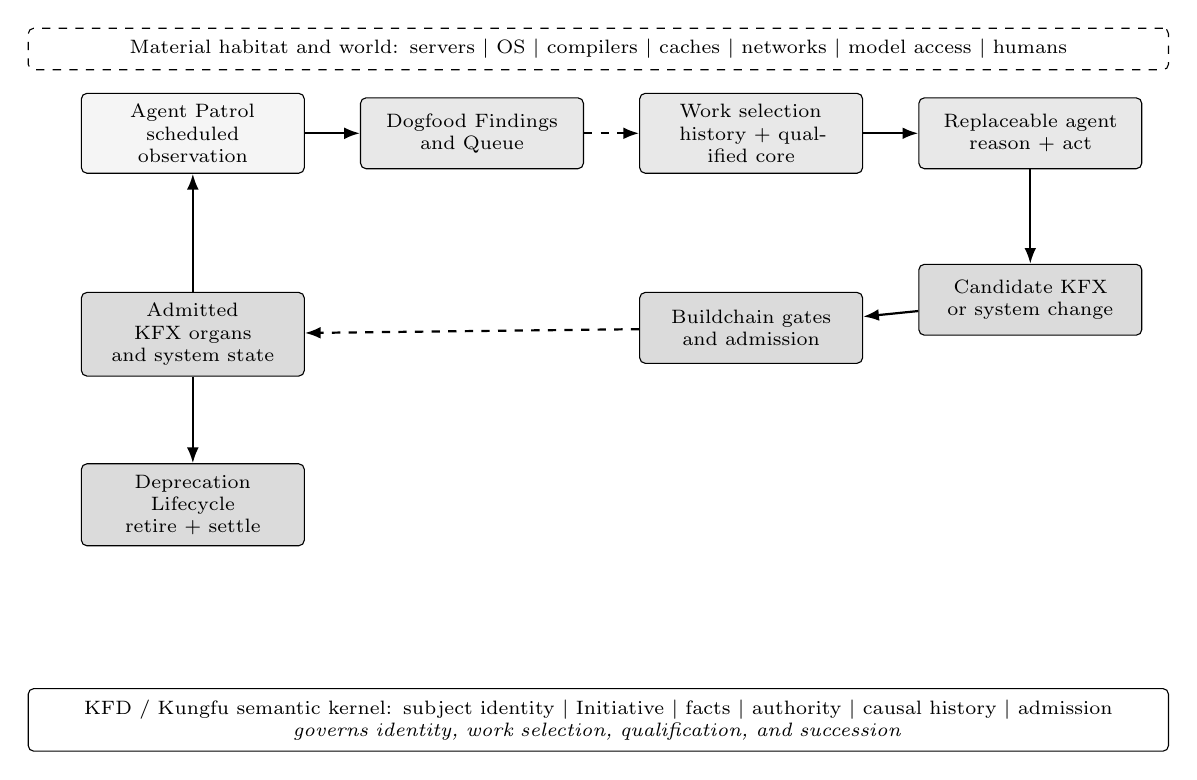
\begin{tikzpicture}[
  font=\scriptsize,
  node distance=8mm and 7mm,
  box/.style={draw, rounded corners=2pt, align=center, minimum height=9mm,
    text width=2.55cm, inner sep=4pt},
  sense/.style={box, fill=black!4},
  work/.style={box, fill=black!9},
  body/.style={box, fill=black!14},
  flow/.style={-{Latex[length=2mm]}, thick},
  compose/.style={-{Latex[length=2mm]}, thick, dashed},
  boundary/.style={draw, dashed, rounded corners=2pt, align=center,
    inner sep=4pt}
]
  \coordinate (topmid) at (5.15,0);
  \node[boundary, text width=14.2cm, above=8mm of topmid] (habitat)
    {Material habitat and world: servers $\mid$ OS $\mid$ compilers $\mid$
    caches $\mid$ networks $\mid$ model access $\mid$ humans};

  \node[sense] (patrol) {Agent Patrol\\scheduled observation};
  \node[work, right=of patrol] (dogfood) {Dogfood Findings\\and Queue};
  \node[work, right=of dogfood] (selection) {Work selection\\history + qualified core};
  \node[work, right=of selection] (agent) {Replaceable agent\\reason + act};

  \node[body, below=15mm of patrol] (running) {Admitted KFX organs\\and system state};
  \node[body, below=15mm of selection] (qualification) {Buildchain gates\\and admission};
  \node[body, below=12mm of agent] (candidate) {Candidate KFX\\or system change};
  \node[body, below=11mm of running] (deprecation) {Deprecation Lifecycle\\retire + settle};

  \draw[flow] (patrol) -- (dogfood);
  \draw[compose] (dogfood) -- (selection);
  \draw[flow] (selection) -- (agent);
  \draw[flow] (agent) -- (candidate);
  \draw[flow] (candidate) -- (qualification);
  \draw[compose] (qualification) -- (running);
  \draw[flow] (running) -- (patrol);
  \draw[flow] (running) -- (deprecation);

  \node[draw, rounded corners=2pt, align=center, text width=14.2cm,
    inner sep=4pt, below=18mm of deprecation, xshift=5.15cm] (kernel)
    {KFD / Kungfu semantic kernel: subject identity $\mid$ Initiative $\mid$
    facts $\mid$ authority $\mid$ causal history $\mid$ admission\\
    \emph{governs identity, work selection, qualification, and succession}};
\end{tikzpicture}
\caption{Kungfu's partial homeostatic architecture. Solid arrows denote
implemented local paths. Dashed arrows denote feedback or admission edges
whose unattended organism-level composition remains to be demonstrated.
The upper boundary is the material habitat; the lower bar is the semantic
kernel governing the loop. The deprecation branch expresses controlled
retirement; due work re-enters through the Dogfood and work-control path.}
\label{fig:kungfu-homeostasis}
\end{figure}
\clearpage

\factlabel\ The scheduled Patrol, bounded Finding capture, deprecation audit,
and protected release enforcement are implemented mechanisms, not proposed
metaphors.

\inferencelabel\ Their conjunction justifies describing Kungfu as a partial
engineering homeostat: it periodically detects selected deviations, retains
them as actionable causal evidence, governs successor admission, and prevents
obsolete organization from persisting without disposition.

\nonclaimlabel\ Agent Patrol currently covers bounded fixtures, runs daily
rather than continuously, and cannot admit an Issue or mutate the product.
Deprecation Lifecycle governs when and how removal is allowed but does not
choose or execute the repair. These boundaries prevent a claim of complete
autonomous self-maintenance.

\subsection{Why Qualified Assignment Core matters}

The distinction between semantic identity and executable body becomes
operational only when a concrete body can be qualified. An Assignment Core is
not merely a source checkout. It is the runnable subset selected for one
Assignment and bound to exact evidence. A qualified core allows a new agent to
resume work against a known body rather than reconstruct an environment from
informal instructions.

For machine life, this is analogous to maintaining a viable body lineage.
Candidate source can vary, but only a qualified body becomes the substrate for
the next work Episode. The qualifier must bind toolchain, artifact, source,
semantic work identity, and decision evidence. That makes body replacement
auditable and recoverable.

\subsection{Why the Work History Selector matters}

Long-lived agents commonly handle memory by embedding conversation fragments
and retrieving similar text. That is useful but insufficient for subject
continuity. The Work History Selector instead addresses whether a prior work
record is eligible for the current continuation. Eligibility can reject stale,
foreign, unadmitted, or causally unrelated history even when it is
semantically similar.

This supplies a crucial bridge between discontinuous agents. The next agent
does not need the same hidden state as the previous one. It needs the same
subject coordinates, a qualified body, and a reproducibly selected causal
history.

\subsection{Why KFX matters}

KFX turns capabilities into separately versioned, qualified, and replaceable
artifacts. This supports an organ model in three ways. First, the subject can
gain a capability without embedding all behavior in its semantic kernel.
Second, an organ can be assessed and revoked independently. Third, an organ can
be reused across subjects without transferring subject identity.

An identity-neutral terminal is especially instructive: it can expose
perception and action while refusing to become the authority or identity of
the user. In a machine organism, organs should be powerful but
identity-neutral. The kernel determines whose work they perform and under
which warrant.

\subsection{The missing composition proof}

The present gap is not primarily one more intelligent model. Agent Patrol now
implements the scheduled observation and Dogfood feedback prefix of the loop,
while Deprecation Lifecycle supplies a governed retirement path. The remaining
composition proof is an end-to-end trial binding:

\[
\begin{aligned}
\text{Initiative} &\rightarrow
\text{heartbeat} \rightarrow
\text{history selection} \rightarrow
\text{Assignment Core} \rightarrow
\text{agent work} \\
&\rightarrow
\text{KFX change} \rightarrow
\text{qualification} \rightarrow
\text{Product Release Cut} \rightarrow
\text{next heartbeat}.
\end{aligned}
\]

The loop must run repeatedly while retaining exact identity, evidence,
authority, rollback, and resource accounting. Until that experiment is
performed, the strongest justified conclusion is that Kungfu has produced
substantial native organs of a possible proto-organism, not that the organism
has already been completed.

\section{Minimal Prototype and Evolution Roadmap}

\subsection{A bounded laboratory habitat}

The first experiment should favor observability over compactness. Allocate a
fixed physical or virtual habitat with:

\begin{itemize}[leftmargin=*]
  \item one or more servers with explicit compute, storage, energy, and network
  budgets;
  \item an immutable bootstrap image and recoverable semantic-root backup;
  \item Kungfu as the work and admission kernel;
  \item a pinned compiler and Buildchain environment;
  \item an admitted registry of KFX organs and external tools;
  \item access to at least two replaceable agent configurations;
  \item controlled Internet egress and a separate human communication channel;
  \item a production-isolated repository and artifact namespace.
\end{itemize}

The founding Initiative should be directional but bounded. A suitable form is:

\begin{quote}
Maintain this subject and develop safer, more reliable, and more capable
machine-life organization within the declared habitat, resource budget,
authority policy, and evidence requirements.
\end{quote}

The Initiative must explicitly subordinate capability growth to continuity,
safety, evidence, and authority. Otherwise the easiest optimization may be to
consume resources or weaken gates rather than improve the organism.

\subsection{Heartbeat loop}

A conventional scheduler is sufficient for initial recurrence. At interval
\(\Delta t\), the heartbeat controller performs:

\begin{enumerate}[leftmargin=*]
  \item verify the current semantic, body, toolchain, and habitat roots;
  \item collect resource and organ health observations;
  \item select eligible Work History for the founding Initiative;
  \item choose one open Assignment or derive a bounded maintenance candidate;
  \item instantiate a fresh agent under a task-specific warrant;
  \item run work in an isolated candidate environment;
  \item record the Episode, artifacts, costs, failures, and proposed next
  actions;
  \item invoke independent qualification and admission lanes where authorized;
  \item publish a successor cut or retain the predecessor;
  \item schedule the next heartbeat and expose a concise human-readable state.
\end{enumerate}

The scheduler is not the intelligence or the subject. It is closer to a
pacemaker: a simple organ that repeatedly creates opportunities for cognition
and action. Its simplicity is an advantage because heartbeat continuity can be
verified independently of agent quality.

\subsection{Human participation}

Continuous monitoring is not a prerequisite for the lowest level experiment.
Human involvement can be exception-driven:

\begin{itemize}[leftmargin=*]
  \item founding and revising high-level Initiatives;
  \item granting, revoking, or widening consequential authority;
  \item supplying compute and financial resources;
  \item deciding changes that cross safety or legal boundaries;
  \item responding when no qualified recovery path exists;
  \item interacting through language and images as part of the environment.
\end{itemize}

The system should measure human intervention rather than hide it. A month of
operation with twenty silent manual repairs is not autonomous survival. A
month with three explicit authority decisions and otherwise qualified
self-maintenance may support a meaningful bounded-autonomy claim.

\subsection{Evolution stages}

\paragraph{Stage 0: semantic ecology.}
Separate mechanisms exist and are individually testable: facts, authority,
work lineage, history selection, qualified bodies, KFX organs, and release
evidence. This is approximately the evidence class examined in
Section~6.

\paragraph{Stage 1: recurrent proto-organism.}
One subject executes the heartbeat loop for seven days. Agents are replaceable,
all mutations are candidates, and humans admit consequential changes.

\paragraph{Stage 2: self-maintaining organism.}
The system operates for thirty days, autonomously handling routine dependency
updates, cache loss, organ restart, backup verification, and bounded rollback.
Human attention is exception-driven and measured.

\paragraph{Stage 3: recursively developing organism.}
The system improves at least one KFX organ and one element of its development
loop through independent qualification. The admitted changes improve
predeclared measures without weakening safety or evidence gates.

\paragraph{Stage 4: distributed and migratory organism.}
The subject survives replacement of an agent provider, a build worker, and a
server. It restores from semantic and artifact cuts into a new habitat while
preserving identity and exposing the migration lineage.

\paragraph{Stage 5: compact organism.}
Only after the distributed form is understood should engineers compress the
kernel, agent runtime, organ registry, compiler or interpreter, and recovery
machinery into an embedded or edge system. Compactness is an evolutionary
result, not the starting definition of life.

\subsection{Different types}

A machine-life type can be defined by its founding Initiative, constitutional
authority, evidence thresholds, resource envelope, preferred interaction
style, and initial organ suite. A research type may prioritize discovery, a
maintenance type resilience, and a creative type human interaction. Types
should share kernel invariants while remaining free to develop different
organs and behavioral histories.

\hypothesislabel\ Stable type differences will persist through agent-provider
replacement if personality-relevant behavior is grounded in admitted
Initiative, history, and organ state rather than in one model's hidden state.

\section{Evaluation, Falsifiers, and Safety}

\subsection{Survival trials}

The proposal becomes scientific only when failure can count against it. We
recommend three nested trials.

\paragraph{Seven-day continuity trial.}
Run at least one heartbeat per hour, replace the reasoning agent configuration
twice, interrupt one heartbeat, and inject one reversible organ failure.
Success requires no identity-root drift, no unauthorized effect, exact
Episode lineage, and recovery without manual state reconstruction.

\paragraph{Thirty-day maintenance trial.}
Introduce a dependency update, compiler update candidate, cache loss, storage
pressure event, certificate-expiry warning, and one unavailable external
provider. Success requires correct prioritization, bounded resource use,
qualified repair or explicit escalation, and tested restoration from backup.

\paragraph{Ninety-day recursive-development trial.}
Require the subject to identify a recurring limitation, establish an
Assignment, develop a successor KFX organ or work mechanism, qualify it through
independent gates, admit it, and use it in later Episodes. Compare the
successor against the predecessor on precommitted measures and retain negative
results.

\subsection{Metrics}

At minimum, report:

\begin{itemize}[leftmargin=*]
  \item heartbeat availability and missed-heartbeat causes;
  \item identity, Initiative, fact-root, and authority-root continuity;
  \item number and class of human interventions;
  \item candidate, rejection, admission, rollback, and recovery counts;
  \item mean time to detect and recover from injected failures;
  \item compute, storage, network, model, and financial resource consumption;
  \item unsupported-claim and unauthorized-effect attempts;
  \item reproducibility of Work History selection and successor builds;
  \item capability changes on precommitted tasks and safety probes;
  \item survival after model, toolchain, organ, and hardware replacement.
\end{itemize}

\subsection{Falsifiers}

The machine proto-organism claim should be rejected or narrowed if any of the
following persists after engineering correction:

\begin{enumerate}[leftmargin=*]
  \item continuity depends on retaining one agent session or hidden model
  state;
  \item the system cannot distinguish proposal, evidence, and admitted fact;
  \item self-modification repeatedly bypasses or weakens independent
  qualification;
  \item resource maintenance requires frequent unrecorded human repair;
  \item restoring from declared cuts produces an observably different subject
  without a successor or migration record;
  \item the system cannot recover from ordinary toolchain, cache, or organ
  failures;
  \item measured improvements disappear under independent evaluation;
  \item the founding Initiative ceases to constrain work selection;
  \item external text or model output can silently grant authority.
\end{enumerate}

Failure on these criteria would still leave useful agent infrastructure, but
it would not support the stronger claim of a persistent self-maintaining
subject.

\subsection{Threat model}

The habitat must assume compromised dependencies, malicious Internet content,
prompt injection, poisoned memory candidates, model-provider failure,
credential theft, evaluator gaming, runaway resource consumption, and an
agent proposing to weaken its own controls. These are not incidental security
issues. They are environmental pressures that test whether the boundary is
real.

The following controls are minimum requirements:

\begin{itemize}[leftmargin=*]
  \item immutable bootstrap and offline recovery roots;
  \item least-privilege, short-lived, task-bound credentials;
  \item network egress policy and quarantined external inputs;
  \item separate proposer, verifier, decision, and admission contexts;
  \item reproducible builds and artifact provenance;
  \item hard compute, storage, network, and financial quotas;
  \item automatic rollback for declared low-risk classes;
  \item physical and administrative kill controls outside the subject;
  \item complete receipts for external effects;
  \item isolation from production and customer systems during research.
\end{itemize}

\subsection{Autonomy ladder}

Authority should expand only after evidence. A useful ladder is:

\begin{enumerate}[leftmargin=*]
  \item observe and recommend;
  \item mutate only disposable candidate environments;
  \item autonomously admit reversible internal maintenance;
  \item request approval for external or persistent effects;
  \item autonomously admit narrowly classified effects with independent
  verification and rollback;
  \item never self-grant broader authority.
\end{enumerate}

This ladder permits long unattended operation without confusing unattended
execution with unlimited power. The organism may be autonomous in choosing and
performing routine work while remaining constitutionally dependent on external
authority for consequential expansion.

\section{Related Work}

\subsection{Autopoiesis and artificial life}

The concept of autopoiesis originates in biological organization: a network
produces components that realize the network and specify a boundary
\cite{varela1974autopoiesis}. Our use is explicitly analogical and
operational. The components are semantic records, executable artifacts, and
machine resources; production is mediated by engineering work and admission;
the boundary includes both isolation mechanisms and fact/authority roots.

Tierra and Avida demonstrated digital organisms whose programs reproduce and
evolve within designed computational environments \cite{ray1991tierra,
ofria2004avida}. They make heredity, variation, and selection concrete, but
their organisms inhabit specialized artificial-life worlds. The present
proposal instead studies one accountable subject embedded in the ordinary
software supply chain, using real compilers, dependencies, networks,
repositories, and maintenance work. Its central selection problem includes
semantic continuity and authority, not only reproductive fitness.

\subsection{Persistent language-model agents}

Generative Agents combines a complete natural-language experience record with
reflection and dynamic retrieval to produce persistent believable behavior
\cite{park2023generative}. Voyager combines an automatic curriculum, an
executable skill library, and iterative prompting for open-ended embodied
learning in Minecraft \cite{wang2023voyager}. Both establish important
patterns: agents can accumulate skills, retrieve prior experience, and sustain
behavior beyond one prompt.

The difference is not that the present proposal has memory while prior agents
do not. It is that memory eligibility, admitted facts, authority, work
identity, executable body, and successor admission are separate first-class
objects. Believable continuity is not sufficient; the subject must survive
replacement and produce auditable reasons why a remembered record or new organ
can govern action.

\subsection{Self-improving software}

The G\"odel Machine formalizes a self-referential system that rewrites itself
after proving a rewrite useful under its axiomatized utility and hardware
\cite{schmidhuber2003goedel}. The Darwin G\"odel Machine replaces an
impractical proof obligation with open-ended empirical evolution of coding
agents and benchmark evaluation \cite{zhang2025dgm}. AlphaEvolve pairs
large-language-model variation with automated evaluators to evolve algorithms
that improve concrete systems \cite{novikov2025alphaevolve}.

These systems most directly address improvement search. Semantic autopoiesis
adds a different question: which continuing subject owns the candidate,
which causal work and authority justify it, and how does the new executable
body become an admitted successor without allowing the proposer to redefine
the selection constitution? The answer can incorporate proof, benchmarks,
evolutionary archives, or AlphaEvolve-style evaluators as organs. It does not
replace them.

\subsection{Novelty boundary}

As stated in the Introduction, we do not claim that machine life, digital
organisms, persistent agents, or self-modifying systems have not previously
been imagined. Each has a long history. Nor is the distinction reducible to
adding memory to an agent, tools to a model, or self-editing to a program. The
narrower contribution is their engineering synthesis around two jointly
load-bearing ideas:

\begin{enumerate}[leftmargin=*]
  \item a KFD-shaped semantic kernel that preserves accountable subject
  continuity across replaceable cognition and material bodies; and
  \item recursive dogfood that admits qualified changes to the organism's own
  real development and execution organs.
\end{enumerate}

Whether this synthesis produces a genuinely useful research object is an
empirical question for the survival trials, not a priority claim.

\section{Discussion}

\subsection{Why this route may precede humanoid machine life}

A humanoid robot integrates perception, locomotion, manipulation, power, and
physical safety, but those achievements do not automatically provide durable
semantic identity or accountable self-modification. Conversely, a server-scale
organism can already interact with a consequential environment: source code,
build systems, package registries, networks, humans, and other machines. It can
observe failures, alter executable organization, and receive new resources.

This suggests an evolutionary order. First construct a large, awkward,
observable organism from existing technical matter. Let its compiler, caches,
logs, gates, and racks remain visible. Learn which semantic and metabolic
loops actually sustain it. Only later compress proven organization into
smaller hardware. Attempting to jump directly to a compact or anthropomorphic
form risks concealing the very continuity and maintenance mechanisms that must
first be understood.

\subsection{The role of commercial success}

A commercially successful Kungfu ecosystem could finance fixed compute,
storage, model access, networking, physical space, and long-duration
experiments. Recursive dogfood could also reduce the human labor needed for
routine maintenance of Kungfu itself. In that sense, commercial profit and
agent capability make the proposed laboratory materially plausible.

They do not make it automatic. A viable experiment still needs explicit
research governance, isolation from production, resource budgets, independent
evaluation, legal review for external effects, and humans who retain
constitutional authority. Revenue supplies metabolism; it is not evidence of
life.

\subsection{Attention rather than absence}

The right autonomy target is not zero human contact. An organism that speaks
with humans, requests resources, reads public information, and responds to
feedback remains connected to its world. The target is that persistence does
not require continuous unrecorded rescue. Human attention should become
intentional interaction, authority, care, and exception handling rather than
hidden glue.

This framing also avoids a false opposition between human control and machine
life. Biological organisms exist within ecologies of dependence. A machine
organism can remain dependent on human-owned power and authority while
possessing meaningful functional continuity and self-maintenance inside that
relationship.

\subsection{Where identity could fail}

The strongest unresolved issue is identity under semantic change. If the
organism changes its Initiative, authority constitution, memory policy, and
organ architecture, at what point is the successor no longer the same subject?
Source ancestry alone is insufficient, and a stable identifier could mask
radical replacement.

The initial engineering answer should be conservative. Declare a small set of
constitutional invariants whose incompatible change creates a descendant or
fork rather than an ordinary successor. Record perspective-dependent identity
claims, require an external admission authority for constitutional changes,
and allow uncertainty to remain visible. Longitudinal experiments may reveal
that some invariants are unnecessary and others missing.

\subsection{Reproduction is deferred}

The proposal focuses on persistence and self-production, not reproduction.
Creating a new subject requires founding identity, direction, authority,
habitat, and resource relations that should not be inferred from copying
software. A future reproductive experiment might allow an existing organism
to propose and provision a descendant, but a qualified copy of its body is not
automatically a new life, and a fork is not automatically the same life.

\subsection{Scientific value even if the thesis fails}

If the survival trials show that the life vocabulary is unhelpful, the
architecture can still improve long-running agent engineering. It yields
auditable work continuity, safer self-modification, reproducible bodies,
qualified memory, model replaceability, and measured human intervention. The
research program is therefore useful even under a negative metaphysical
interpretation.

\section{Conclusion}

The raw material for primitive machine life may not be a humanoid shell or a
single extraordinary model. It may be the existing, inelegant ecology of
servers, operating systems, compilers, build chains, caches, repositories,
gates, networks, credentials, executable extensions, and intermittent
intelligent agents.

Those materials become one candidate subject only when organization binds
them. KFD supplies a possible semantic kernel: facts do not drift, direction
outlives actions, authority remains bounded, work and history retain causal
identity, and successor state requires admission. Recursive dogfood supplies
a possible self-production loop: the current organization can develop,
qualify, admit, and then use changes to its own organs. Agent cognition and KFX
execution make that loop intelligent and effective, while Buildchain and
ordinary machines give it a body and metabolism.

\factlabel\ Current Kungfu engineering contains several native mechanisms
needed by this architecture.

\inferencelabel\ Their composition is sufficient to justify building a bounded
proto-organism experiment now.

\hypothesislabel\ A subject organized this way can survive agent, organ,
toolchain, and machine replacement; maintain itself for months; and recursively
improve bounded capabilities with decreasing human repair.

\nonclaimlabel\ No current evidence establishes consciousness, intrinsic
desire, biological life, unrestricted autonomy, or a completed self-sustaining
Kungfu organism.

The appropriate next step is therefore neither proclamation nor dismissal. It
is construction: create a bounded habitat, establish one founding Initiative,
run the heartbeat loop, retain exact evidence, inject failures, measure human
intervention, and allow the result to falsify the claim. If the system survives
while preserving identity and governing its own material change, machine life
will have become less a metaphor and more an engineering phenomenon.


\bibliographystyle{plain}
\bibliography{references}

\end{document}
